

\tikzset{every picture/.style={line width=0.75pt}} %set default line width to 0.75pt        

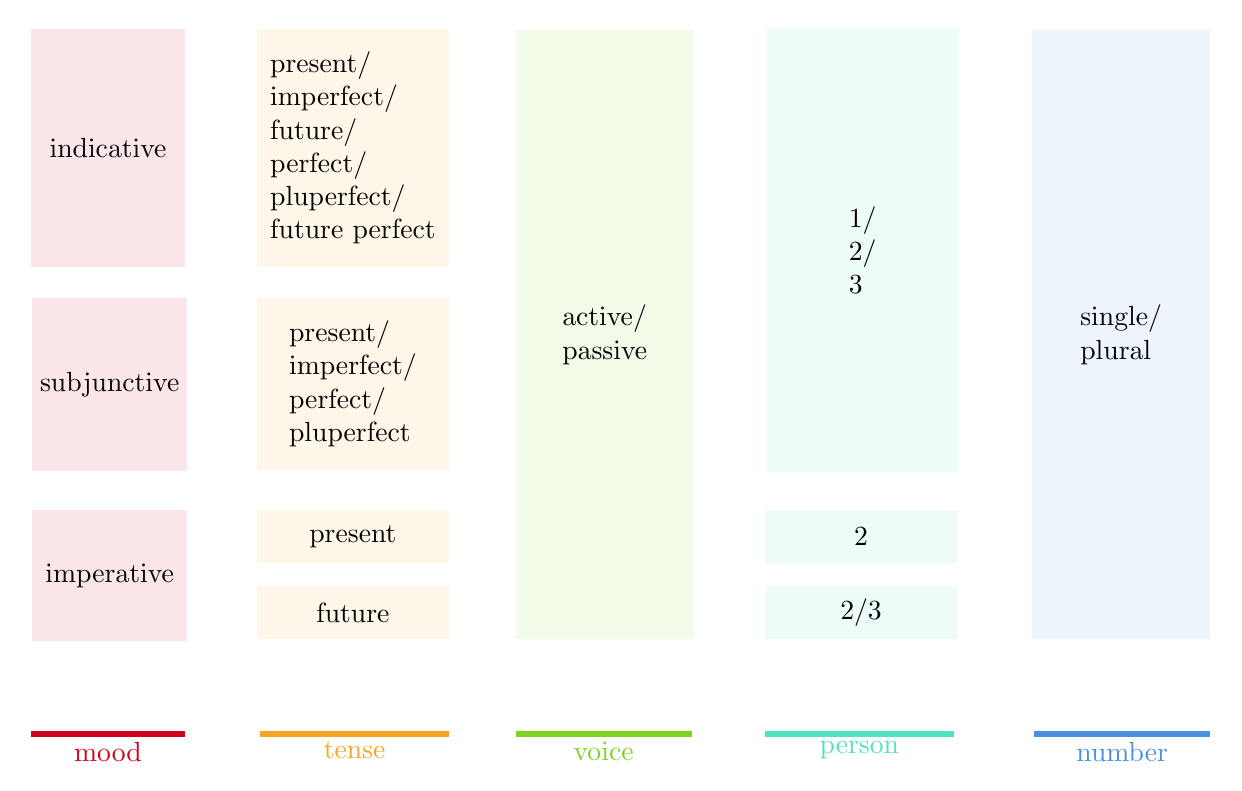
\begin{tikzpicture}[x=0.75pt,y=0.75pt,yscale=-0.8,xscale=0.8]
%uncomment if require: \path (0,560); %set diagram left start at 0, and has height of 560

%Straight Lines [id:da4771979505475994] 
\draw [color={rgb, 255:red, 208; green, 2; blue, 27 }  ,draw opacity=1 ][line width=2.25]    (72,476.59) -- (165,476.59) ;
%Shape: Rectangle [id:dp4651809120211663] 
\draw  [draw opacity=0][fill={rgb, 255:red, 208; green, 2; blue, 27 }  ,fill opacity=0.1 ] (72,51.93) -- (165,51.93) -- (165,195.59) -- (72,195.59) -- cycle ;
%Shape: Rectangle [id:dp8674436914111818] 
\draw  [draw opacity=0][fill={rgb, 255:red, 245; green, 166; blue, 35 }  ,fill opacity=0.1 ] (208,51.93) -- (324,51.93) -- (324,195.59) -- (208,195.59) -- cycle ;
%Straight Lines [id:da9097932489630769] 
\draw [color={rgb, 255:red, 245; green, 166; blue, 35 }  ,draw opacity=1 ][line width=2.25]    (210,476.59) -- (324,476.59) ;
%Shape: Rectangle [id:dp6458311390526075] 
\draw  [draw opacity=0][fill={rgb, 255:red, 245; green, 166; blue, 35 }  ,fill opacity=0.1 ] (208,213.93) -- (324,213.93) -- (324,317.59) -- (208,317.59) -- cycle ;
%Shape: Rectangle [id:dp4418485190624626] 
\draw  [draw opacity=0][fill={rgb, 255:red, 208; green, 2; blue, 27 }  ,fill opacity=0.1 ] (73,213.93) -- (166,213.93) -- (166,318.26) -- (73,318.26) -- cycle ;
%Shape: Rectangle [id:dp7155013561532602] 
\draw  [draw opacity=0][fill={rgb, 255:red, 245; green, 166; blue, 35 }  ,fill opacity=0.1 ] (208,341.59) -- (324,341.59) -- (324,373.59) -- (208,373.59) -- cycle ;
%Shape: Rectangle [id:dp5109073549880265] 
\draw  [draw opacity=0][fill={rgb, 255:red, 245; green, 166; blue, 35 }  ,fill opacity=0.1 ] (208,387.59) -- (324,387.59) -- (324,419.59) -- (208,419.59) -- cycle ;
%Shape: Rectangle [id:dp4978185928249894] 
\draw  [draw opacity=0][fill={rgb, 255:red, 208; green, 2; blue, 27 }  ,fill opacity=0.1 ] (73,341.59) -- (166,341.59) -- (166,420.93) -- (73,420.93) -- cycle ;
%Shape: Rectangle [id:dp7974586880324295] 
\draw  [draw opacity=0][fill={rgb, 255:red, 126; green, 211; blue, 33 }  ,fill opacity=0.1 ] (364,52.93) -- (471.33,52.93) -- (471.33,419.59) -- (364,419.59) -- cycle ;
%Straight Lines [id:da40576537799721035] 
\draw [color={rgb, 255:red, 126; green, 211; blue, 33 }  ,draw opacity=1 ][line width=2.25]    (364,476.59) -- (470,476.59) ;
%Shape: Rectangle [id:dp37304865952309374] 
\draw  [draw opacity=0][fill={rgb, 255:red, 80; green, 227; blue, 194 }  ,fill opacity=0.1 ] (515,51.93) -- (631,51.93) -- (631,318.93) -- (515,318.93) -- cycle ;
%Shape: Rectangle [id:dp09424442237743991] 
\draw  [draw opacity=0][fill={rgb, 255:red, 80; green, 227; blue, 194 }  ,fill opacity=0.1 ] (514,341.59) -- (630,341.59) -- (630,373.59) -- (514,373.59) -- cycle ;
%Shape: Rectangle [id:dp7879043441622926] 
\draw  [draw opacity=0][fill={rgb, 255:red, 80; green, 227; blue, 194 }  ,fill opacity=0.1 ] (514,387.59) -- (630,387.59) -- (630,419.59) -- (514,419.59) -- cycle ;
%Straight Lines [id:da6694037096709569] 
\draw [color={rgb, 255:red, 80; green, 227; blue, 194 }  ,draw opacity=1 ][line width=2.25]    (514,476.59) -- (628,476.59) ;
%Shape: Rectangle [id:dp8356914669291959] 
\draw  [draw opacity=0][fill={rgb, 255:red, 74; green, 144; blue, 226 }  ,fill opacity=0.1 ] (675,52.93) -- (782.33,52.93) -- (782.33,419.59) -- (675,419.59) -- cycle ;
%Straight Lines [id:da18180972606397305] 
\draw [color={rgb, 255:red, 74; green, 144; blue, 226 }  ,draw opacity=1 ][line width=2.25]    (676.33,476.59) -- (782.33,476.59) ;

% Text Node
\draw (118.5,123.76) node   [align=left] {indicative};
% Text Node
\draw (119.5,266.09) node   [align=left] {subjunctive};
% Text Node
\draw (266,123.76) node   [align=left] {present/\\imperfect/\\future/\\perfect/\\pluperfect/\\future perfect};
% Text Node
\draw (266,265.76) node   [align=left] {present/\\imperfect/\\perfect/\\pluperfect};
% Text Node
\draw (417.67,236.26) node   [align=left] {active/\\passive};
% Text Node
\draw (573,185.43) node   [align=left] {1/\\2/\\3};
% Text Node
\draw (728.67,236.26) node  [color={rgb, 255:red, 0; green, 0; blue, 0 }  ,opacity=1 ] [align=left] {single/\\plural};
% Text Node
\draw (119.5,381.26) node   [align=left] {imperative};
% Text Node
\draw (266,357.59) node   [align=left] {present};
% Text Node
\draw (266,403.59) node   [align=left] {future};
% Text Node
\draw (572,357.59) node   [align=left] {2};
% Text Node
\draw (572,403.59) node   [align=left] {2/3};
% Text Node
\draw (118.5,479.59) node [anchor=north] [inner sep=0.75pt]  [color={rgb, 255:red, 208; green, 2; blue, 27 }  ,opacity=1 ] [align=left] {mood};
% Text Node
\draw (267,479.59) node [anchor=north] [inner sep=0.75pt]  [color={rgb, 255:red, 245; green, 166; blue, 35 }  ,opacity=1 ] [align=left] {\textcolor[rgb]{0.96,0.65,0.14}{tense}};
% Text Node
\draw (417,479.59) node [anchor=north] [inner sep=0.75pt]  [color={rgb, 255:red, 126; green, 211; blue, 33 }  ,opacity=1 ] [align=left] {voice};
% Text Node
\draw (571,479.59) node [anchor=north] [inner sep=0.75pt]  [color={rgb, 255:red, 80; green, 227; blue, 194 }  ,opacity=1 ] [align=left] {\textcolor[rgb]{0.31,0.89,0.76}{person}};
% Text Node
\draw (729.33,479.59) node [anchor=north] [inner sep=0.75pt]  [color={rgb, 255:red, 74; green, 144; blue, 226 }  ,opacity=1 ] [align=left] {number};


\end{tikzpicture}
